% \chapter{Introduction to Analysis}
% {\color{red} having introduced the model, we will now analyze it. We will begin with a basic calibration of the 
% First we'll show the result of the base model for the shift in the ownership and class structure in the city. After that, we'll do 
% The idea is that there is wealth created in the city, 
% This is what you expect to see in terms of the ownership
% What if financialization actually changes the urban agglomerations effect.
% One is whether it could feed back and effect the productivity.
% IT turns out there are effects on the productivity. 
% The other is 
% What would that mean and how would you model that. }





\chapter{The Transmission Puzzle} \label{chapter-tramsmission}%{Distribution and Growth} \label{chapter-distribution}
% \chapter{Productivity Spillovers} \label{chapter-productivity-spillovers}

\epigraph{Alternative micro-foundations cannot be regarded as interchangeable contents for the black box \dots %The micro-foundations of urban agglomeration economies interact with other building blocks of urban models in ways that we cannot recognise unless they are explicitly stated. For instance, the composition of cities typically emerges as a consequence of the scope of different sources of agglomeration economies and their interaction with other aspects of individual behaviour. Third, 
different micro-foundations have different welfare and policy implications. %If we begin building an urban model by postulating an aggregate production function with increasing returns, we can only take this function as given. If instead we derive this aggregate production function from first principles, we may see that its efficiency can be improved upon. The means for achieving such an improvement will depend on the specifics of individual behaviour and technology. Thus, while different assumptions regarding individual behaviour and technology may support similar aggregate outcomes, the normative implications of alternative micro-foundations can differ substantially.
}{Duranton and Puga \cite{durantonMicroFoundationsUrbanAgglomeration2004}}

\epigraph{A large body of literature documents the existence of agglomeration economies in developed economies ... The main conclusion of this literature is the finding of scale economies of 3--8 percent (that is, a 10 percent increase in the size of an activity in a city raises productivity in this activity by 0.3--0.8 percent).}{Gilles Duranton \cite{durantonAreCitiesEngines2009}} % (see Rosenthal and Strange 2004 for a review).





{\color{black} In Chapter~\ref{chapter-growth} we showed that two lines of research, growth theory and work on urban scaling, have settled on one of the most robust ``stylized facts'' in economics: wealth scales superlinearly with density. However, there is variation between regions that has not yet been adequately explained.\footnote{Although research consistently finds strong agglomeration effects, there is a great deal of variation in the estimates.McCoskey and Kao \cite{mccoskeyPanelDataInvestigation} show that the impact of urbanization on growth varies greatly among countries, however. The World Bank (2016), for example, reported that every 1\% growth in urban population correlates with an increase in GDP per capita by 13\%, 1
0\%, and 7\% in India, China, and Thailand, respectively. Indonesia realizes only 4\% GDP growth for every 1\% increase \cite{haryantotriRelationshipUrbanizationEducation2021}.  The literature has not yet settled on an explanation of the variation.  \cite{loboUrbanScalingProduction2013, pugaMagnitudeCausesAgglomeration2010} } There is speculation that financialization may be a factor in this variation. 

Our model illustrates the mechanism by which financialization captures the value produced in cities by agglomeration effects. This affects wealth distribution because it is specifically shifting flows of capital to financial actors. If financialization is contributing to the variation in wealth production noted empirically, it could be because the shift in ownership has effects on the productivity of the city itself. In this chapter, we will explore that possibility}

Substantial empirical research has shown that the general relationship  between population and output at the urban %is well approximated by 
follows Equation~\ref{eq-agglom-eqn2}: \cite{loboUrbanScalingProduction2013}.\footnote{We use $\beta$ here because it is the most common form in the literature on urban agglomeration, although elsewhere we use $\gamma$, $\alpha$ and $\beta$ for the coefficients on capital and labour respectively as is most common in the economics literature.}

\begin{equation}\label{eq-agglom-eqn2}
    Y=AN^\beta,\qquad \beta>1. 
\end{equation}
There may be multiple and variable channels that link financialization to the magnitude of agglomeration effects in different regions. 
The simplest link can be made through the scale parameter $A$, which controls the overall productivity of the urban system. It captures several productivity enhancing effects: the contribution of urban infrastructure, ownership participation by residents, local investment in productive capital, regulatory structure, the presence of local universities, the skill level of the workforce, as well as other factors. 
Since we are interested in the effect of financialization and ownership, we rewrite $A$ as
\[ A= A_0 + share * rent\]
$A_0$ represents outside or general factors contributing to productivity, while $share*rent$ stands for the share of the urban locational rents captured by residents contributing to local productivity\footnote{that there are local factors is indicated by the variability of estimates of $A$ in empirical studies. See Subsection~\ref{fig/sec-fig-resiudals}.}. The share term is itself a composite of the actual land-ownership share of residents determined by the housing market and the propensity to invest locally.  It might contribute to overall productivity through several channels we discuss below:  directly through investments that raise productivity in firms, indirectly through investments in urban infrastructure such as transportation that cuts production, or through other channels such as workforce improvements. 

A simulation of this linkage is illustrated in Figure~\ref{fig-impact-channel-example}. The finance-driven change in ownership share shown in the lower panel transforms  a city of homeowners  into a city of renters over the course of a lifetime. It also has, as we hypothesize,very large economic implications. The change in the the class structure of the city induces a decline in worker productivity and capital investment, result in in reduced firm size and the number of firms, as well as an overall reduction in population. Declining productivity is the primary channel, which pulls down the wage and the other population variables. The change is amplified by the resulting reduction in  aggregation effects. effects.  exist. This is a much poorer society  as a result of financialization if the linkages we have hypothesized exist.  We do not have empirical estimates the strengths of the channels through which the productivity effect would work, so only the direction of the impacts illustrated should be taken seriously.  

\begin{figure}[h!tb]\label{fig-impact-channel-example}
    \centering
    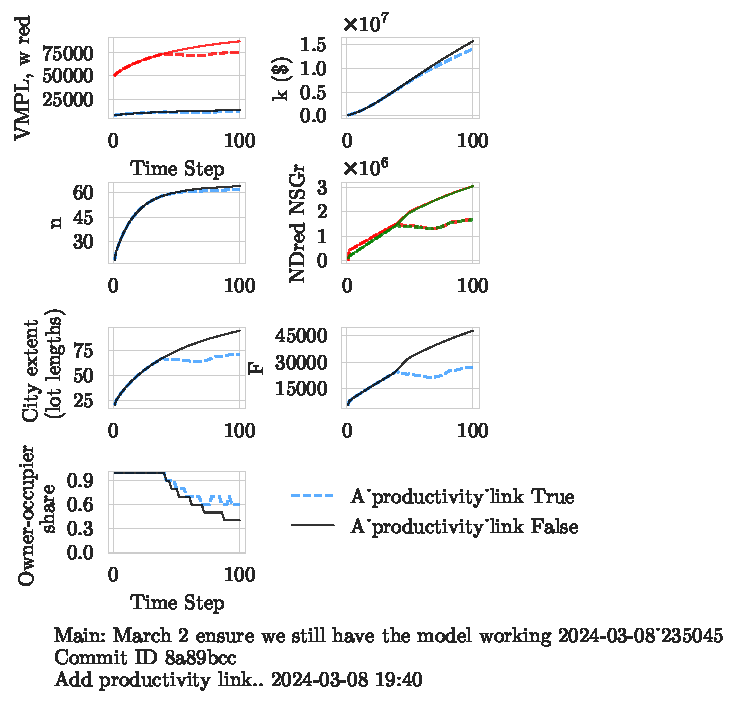
\includegraphics[scale=1, trim=.25cm 2cm .25cm .25cm, clip]{fig/productivity_link.pdf}
    \caption{Illustrating the impact of financialization on an urban economy}
\end{figure}
This is, to our knowledge, a new result, although it is consistent with fundamental urban theory and with The trends we see today in the urban system. The genuinely new component in our result is the formal  linkage of the financialized housing market to  urban productivity.

\subsubsection{Policy implication}
Assuming there are linkages of the sort we have illustrated here, it is important to ask if there are policy implications. Figure~\ref{Productivity_link_and_CG} indicates the effect of a 100\% capital gains tax on land speculation. 

\begin{figure}[h!tb]\label{fig-Productivity_link_and_CG}
    \centering
    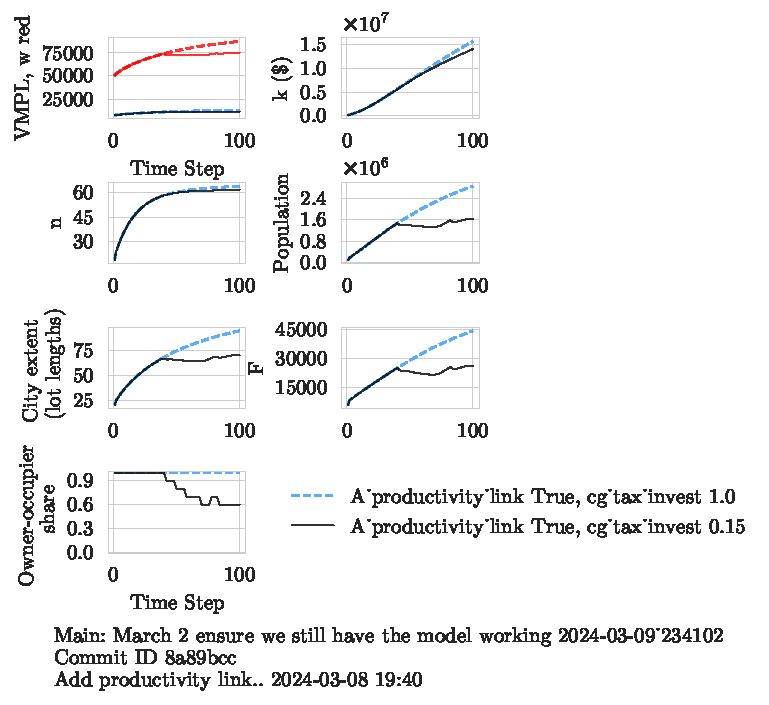
\includegraphics[scale=1, trim=.25cm 2cm .25cm .25cm, clip]{fig/Productivity_link_and_CG.pdf}
    \caption{The corrective effect of a capital gains tax}
    \label{fig:Productivity_link_and_CG}
\end{figure}

The figure shows that a 100\% capital gains tax on land speculation returns the city to its pre-financialization path, indicated by the solid line. In the housing market it has An `excess' effect, eliminating investor participation in the market, shown by the dashed line, and leading to higher rates of home ownership. 

% {\newpage\thispagestyle{empty}
% \vspace{-1.5cm}
\begin{figure}[h!tb]\label{fig-impact-channels}
%\vspace{-1cm}
\begin{adjustwidth}{-0.24\textwidth}{-0.24\textwidth}
\centering
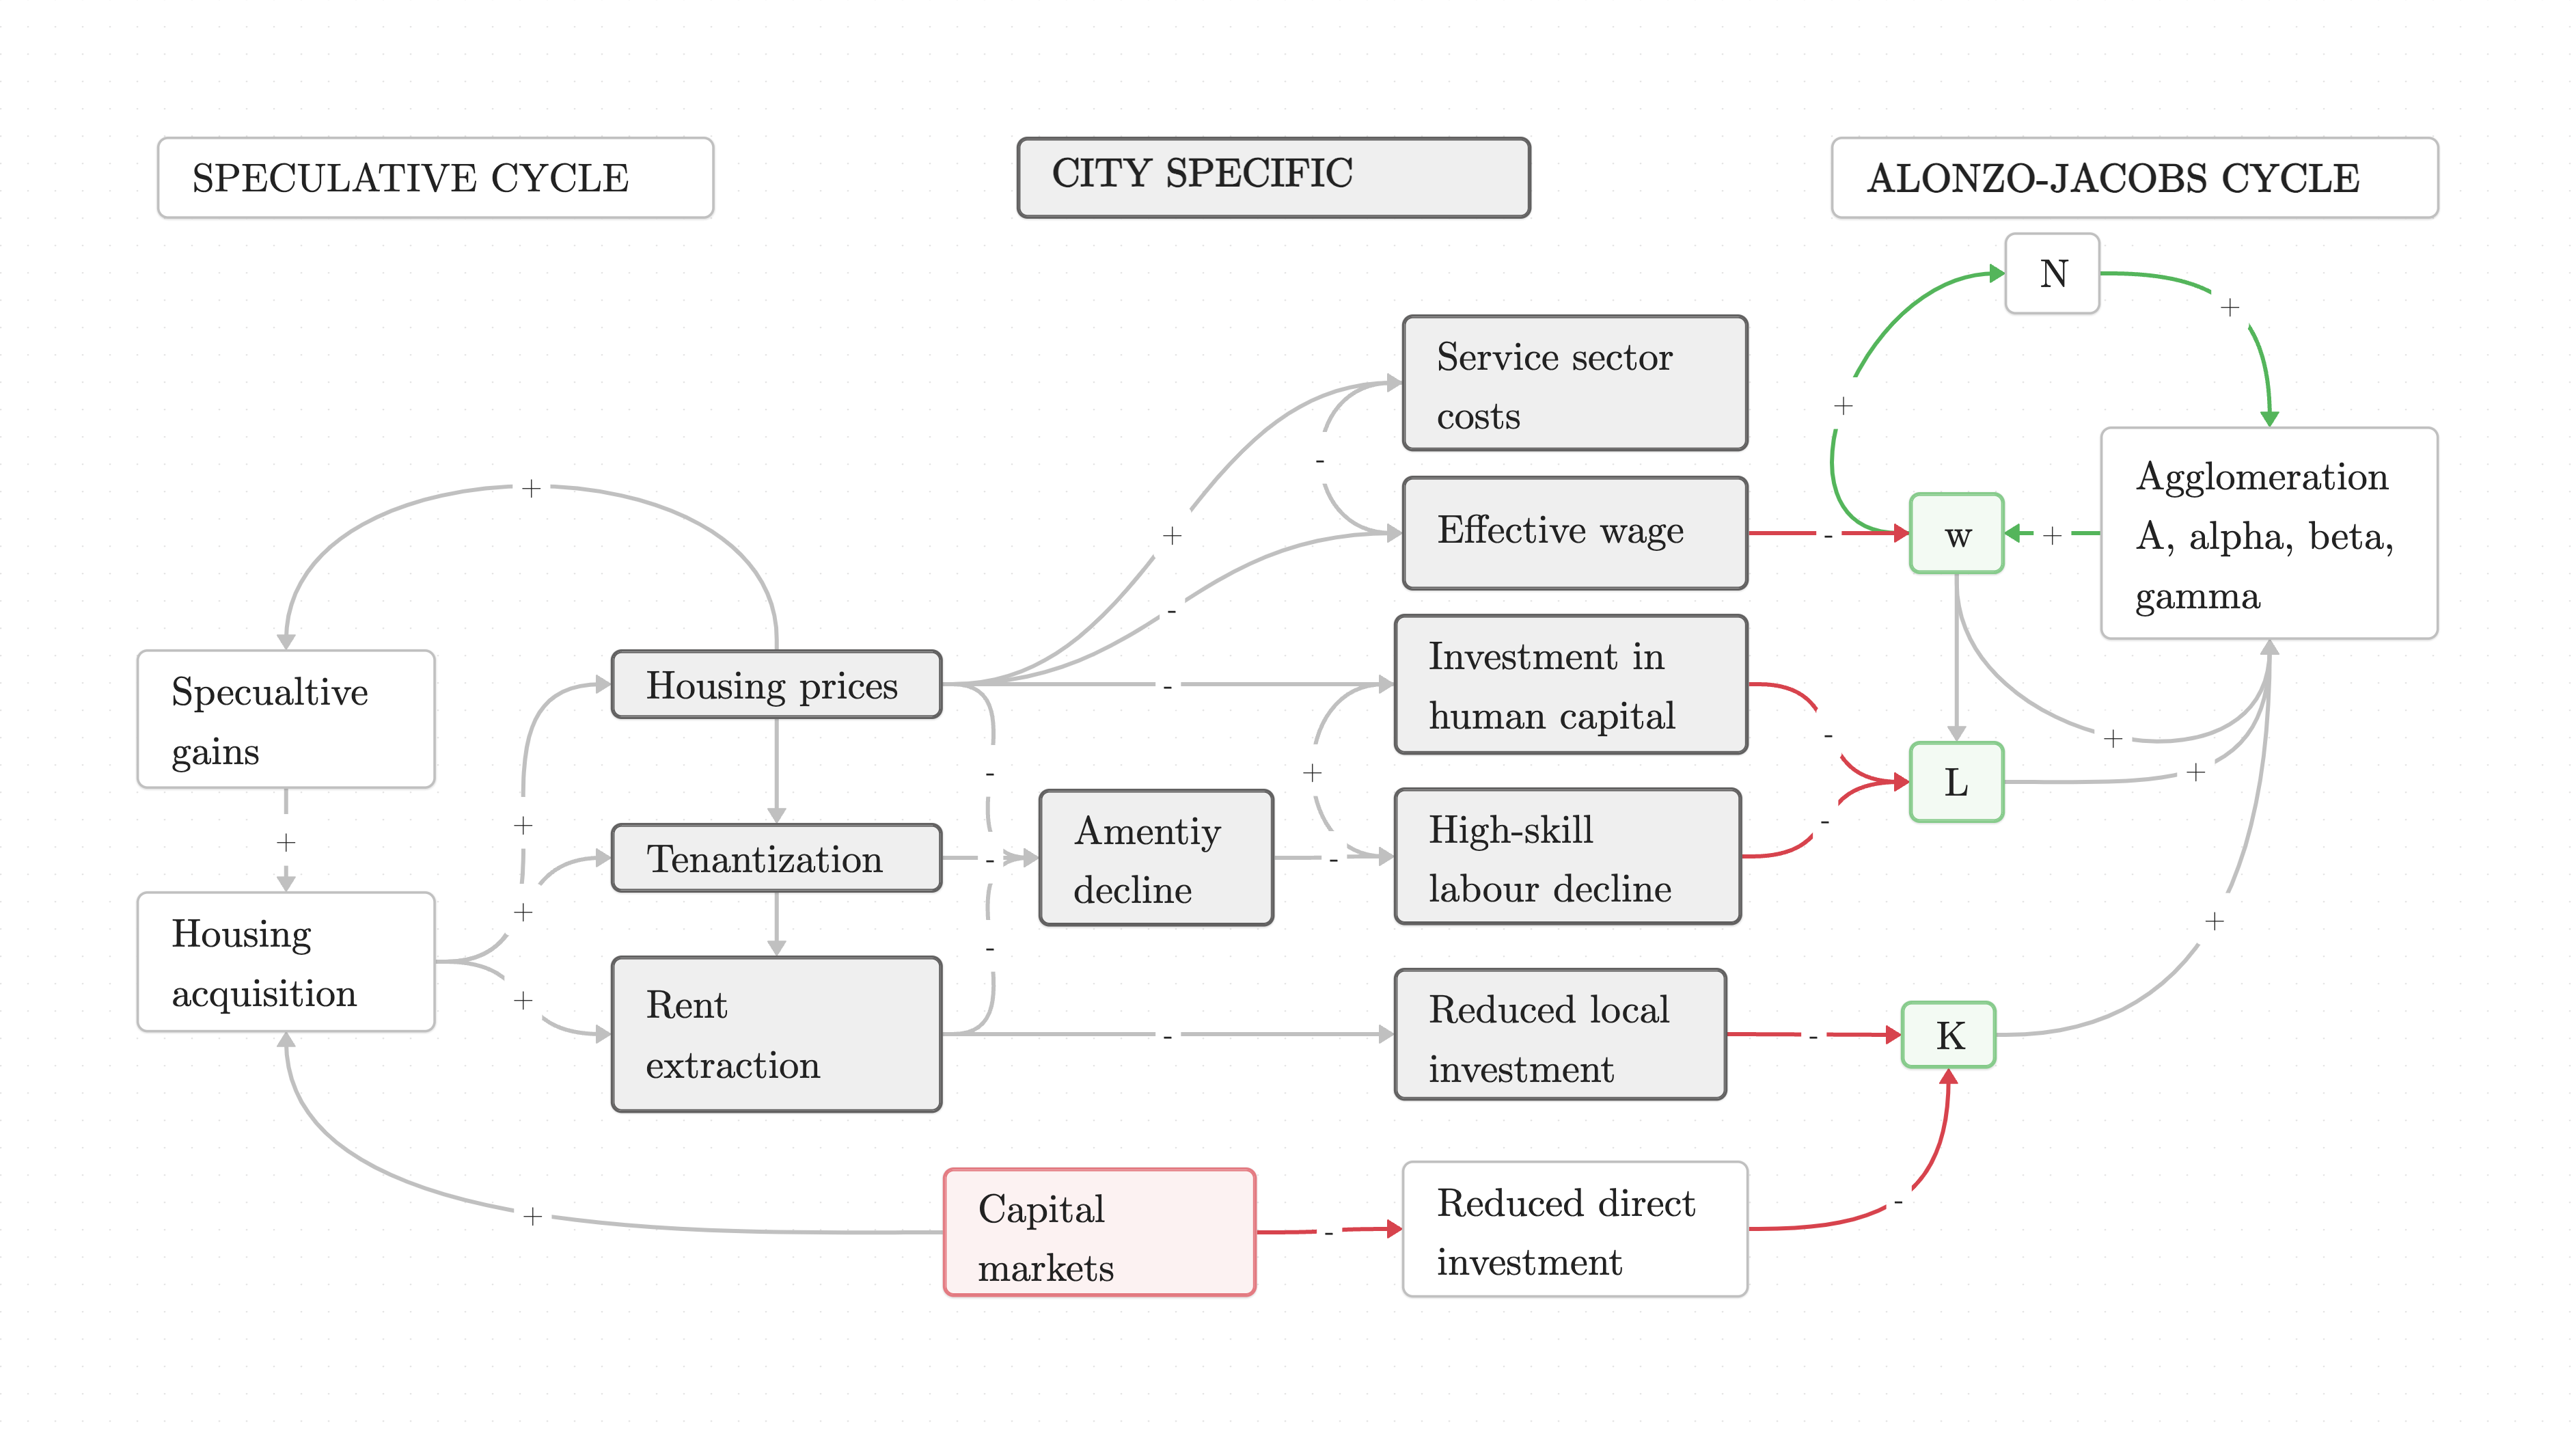
\includegraphics[scale=.15 ]{fig/impact-channels.png}%angle=90
\end{adjustwidth}
\caption{Impact channels relating financialization and urban productivity.}
\end{figure}
%}
 
%In addition, the variation suggests that that financialization may have an impact through multiple channels.  

% the channels through which the effect works are not clearly understood. 

% In particular, how the changes induced by financialization of the housing market might affect the fundamental productivity of the city has not been explored.



%{\color{red} In the next section we discuss potential linkages  with reference to the two dominant theoretical frameworks for understanding agglomeration effects, %. Second, it introduces the micro-foundations, the mechanisms by which agglomeration happens, drawing on the literature, and discussing how financialization might affect those mechanisms. Finally, in section~\ref{section-impact-channel-summary}, we summarize the primary linkages as they might appear in our model.} 

\section{Impact channels}
In the previous  section we  used our model to explore some  implications of a hypoithetical link between financialization of an urban housing market urban and the urban production economy. We now discuss in some detail the impact channels through which financialization. actually works. 

Understanding the mechanisms has considerable policy importance because it raises the possibility that there are several channels for public policy to enhance the positive effects of agglomeration. If the agglomeration parameters $A$ and  $\beta$ can be affected positively by policy choices, or perhaps negatively by trends such as financialization,  governments may be able to significantly increase social wealth and well-being. We discuss potential channels more fully in the following sections. 

Determining the importance of the various impact channels in general or for a specific city is an empirical problem well outside the brief of this thesis. Tests in the universe of the model, however, can lay the foundation for later empirical work. Identifying channels through which the policies or trends might affect productivity is important for this work because by introducing hypothesized linkages into our model explicitly, we have created a framework for systematically testing the model's sensitivity to a range of policy interventions. 

Figure~\ref{fig-impact-channels} illustrates some of the channels through which the financialization of housing might impact city productivity. 
In the figure, the production sector is on the right, the processes occurring within the city are central, and the speculative intervention in the housing market is to the left.  \footnote{The figure only shows some of the links and feedbacks we discuss. It is not our intent in this chapter to provide  a comprehensive discussion of any of the linkages we examine. Each of the linkages shown or mentioned warrants extensive research, and for most even a brief literature search will reveal many related papers.} 


In the upper right, we show the \gls{Alonzo-Jacobs cycle}, described in Chapter~/ref{chapter-model}. In it, the strength of the agglomeration effect determines productivity, which drives wages, which determines population which feeds back to agglomeration. In our model, anything that affects productivity must affect this cycle directly or indirectly.  We show the effect of interventions or financialization on productivity primarily through their effect on wages, labour supply and capital supply. %making it indistinguishable from the Jacobs model at the urban level. 

 %Identifying these linkages is important but it is complicated on at least two levels. First, the micro-level mechanisms driving productivity gains in the production sector, themselves are not well understood.  Second, the linkages between urban productivity and financialization have not been established.  

% {\color{red}
% \section{Mechanisms by which Financialization affects Productivity}
% The literature identifies several possible mechanisms by which financialization might feed back into affecting the productivity of the city. ANY THING OVERARCHING WE CAN SAY ABOUT THIS?LATER, IN CONCLUSION YOU SAY : To do this, we identified the housing market channels through which the changes in ownership might be transmitted through the economic and social body of of the city to the Alonso-Jacobs cycle, where agglomeration effects generate wealth.  }

\subsection{Reduced capital stock}

Marxist theorists \cite{lefebvreRevolutionUrbaine1970, harveyClassmonopolyRentFinance1974, harveyUrbanProcessCapitalism1978, christophersRevisitingUrbanizationCapital2011} have argued that finacialization diverts capital investment from productive investment to financial enterprises. 

This direct effect is illustrated at the bottom of Figure~\ref{fig-impact-channels}, where capital markets can divert capital from the productive activities on the right to speculative activities on the left.  Switching happens in response to the relative rates of return on the two sides. We have assumed a perfectly elastic supply of capital to firms and speculators, leaving modelling more complex and possibly more realistic capital markets to later work.  We allow the rate of return on housing investment to rise in response to city growth, however, attracting speculative investment. We could also simulate a falling rate of return on non-housing investment by reducing the cost of capital to investors or by inhibiting the rate of growth of capital on the production side in response to rising investment in housing purchases. % adjK



\subsection{Local investment}

Financialization may reduce the amount of local capital available, raising the cost of capital in the city. 
There are at least two mechanisms by which local investment capital may be affected. First, if increased tenantization and rent extraction reduce household wealth, we would expect household investment to decline. The decline would probably be correlated with a decline in direct investment, amplifying its effect. Furthermore, this channel would act very slowly and persist after an initial round of speculative activity. 

Second, because private production is complemented by public infrastructure, it is possible that the tenantization for the city would lead to declining municipal investment in public infrastructure. It is known, however, that municipalities generally spend less on tenants and collect more revenue per capita from rental as opposed to owner-occupied housing, so tenatization might lead to rising pressure for infrastructure expenditure.  We can capture these effects by linking the owner-occupier ratio to capital stock. A more detailed approach would explicitly allocate some of the municipal taxes to increasing the agglomeration parameters. 




\subsection{High-skill labour decline}

 Speculation and rising housing prices that result in tenantization will make a city less attractive to highly skilled labour, making it more difficult to attract or hold people with the specific adaptive skills Glaeser and Saiz \cite{glaeserRiseSkilledCity2003} identified. Slowing in-migration or increasing out-migration of the more skilled members of the labour force  will \textit{ceteris paribus} reduce the effective supply of labour. 
Liu et al \cite{liuImpactUrbanHousing2023}, for example, found for China that and increase in urban housing prices has a crowding-out effect on labour mobility.  Duffy et  \cite{duffyRisingHousePrices2005} found that for Ireland that rising house prices, by discouraging potential migrants, could significantly reduce the growth potential of the economy, shifting the balance of labour market growth from employment to wages, with a consequent deterioration in competitiveness. %Anecdotal evidence comes from comes form the frequent news stories about which cities are most livable: low housing prices are almost always an important element in the measures used. (we omit the link form  housing prices to high-skill labour. 

Althobaiti et al \cite{althobaitiHousingPricesSkills2021}  show that with gentrification, high-level cognitive skills are getting closer to the city center in response to the increase of median housing prices while low-level physical skills got further away.  Gentrification can be seen as trend opposing tenantization. The effects of tenantization, neighborhood decline and disinvestment, which Cornelissen and Jang-Trettien \cite{cornelissenHousingContextNeighborhood2023} point  are more common than gentrification in low-income neighborhoods, are likely to be opposite of the effects of  gentrification.

The reduction might be offset by importing human capital, though immigration or rising wages for talent in the city. Florida\cite{floridaCompetingAgeTalent2005, floridaCreativeClassEconomic2014} has suggested that urban growth is strongly linked to the ability to attract talent. 

We can introduce this channel by making  the labour elasticity of output in the Cobb-Douglas function, $\beta$, depend on the home-ownership ratio.  


\subsection{Reduced investment in human capital}

There is a vast literature on investment in human capital. 
Growth theory associates increasing returns to scale in the industrial sector or at the national level with increasing effective human capital, which grows faster than the labour supply as a result of increased education, as we described in Chapter~\ref{chapter-growth} section~\ref{section-growth}. 
Growth theory suggests that the growth of human capital is  a major driver of productivity.  At the national level, Solaki \cite{solakiRelationshipEducationGDP2013} demonstrates a causal relationship between education and growth, and that tertiary Education should be considered as an exogenous variable.  Empirical results for Bangladesh \cite{islam2007relationship}show evidence of bidirectional causality between education and growth.  Among others, B\"uchler et al have recently confirmed the important of human capital growth for urban growth.

There are at least two mechanisms by which investment in human capital may be affected indirectly by financialization. The most direct is by reducing household incomes The effect may be different for different parts of the population. Increasing housing prices increases the wealth of owner-occupiers. this wealth effect may result in increased spending on education for offspring. Increased housing costs for tenants, on the other hand,  may result in reduced human capital investment.\footnote{Glaeser and Saiz found evidence for skill upgrading in declining cities, which suggested to them efficient investment in less skilled workers is a key adaptive/growth mechanism. If powerful enough this effect might offset some of the negative impacts of financialization we has suggested.}  

Less directly, we suspect financialization will increase the cost of living through, for example, increasing labour costs in the service sector. This results in a reduction of the effective wage, also reducing income available for human capital investments. Rent capture leading to reduced local capital of reinvestment in human capital might reduce the adaptive capacity of a city's population.

We can simulate some human capital effects simply by making a link from the home-ownership ratio to the productivity parameters  $\beta$ and $A$. 



\subsection{The effective wage}

Purchasing power depends on the money wage and on the price level. inflation coming from the right side of the figure will reduce the effective urban wage, which Lobo et al. find is one of the determinants of growth. 

 Rising housing prices and rising rental prices reduce the purchasing power of city dwellers in more than one way. In addition to the direct effect, the rising housing costs make other goods and services more expensive. The wage of the Barista must go up, so the cost of a coffee has to rise. Bookstores may close, reducing the neighbourhood amenity level. 
 
 Local amenities may also be affected. Urban amenities  are part of the incentive for choosing city life for many, and any decline in amenity will have the same qualitative effect as a decrease in the wage. The size of the effect will vary because people's tastes differ. 


 General financialization may also reduce the bargaining power of labor, as Tomaskovic-Devey and Lin argue \cite{tomaskovic-deveyFinancializationCausesInequality2013}, reducing wages.\footnote{Tomaskovic-Devey and Lin point to a shift in behaviour of non-finance firms away from production and non-financial services and toward financial investments and services. This shift, they argue,  has led to lower employment, income transfers to executives and capital owners, and increased inequality among workers \cite{tomaskovic-deveyFinancializationCausesInequality2013}}
%In the second part of the chapter we implement several of the mechanisms and share results. 

% VERY INTERESTING \cite{buchlerImpactHumanCapital2024} in areas with elastic housing supply, the positive demand shock leads to the construction of more housing, a larger labour force, and, thus, moderate wage growth. In contrast, in areas of low housing supply, the positive demand shock has a limited impact on new housing construction and the urban population. Human capital gets capitalised into higher home prices, hindering urban growth.

\subsection{The amenity channel}
Rent capture might influence the concentration of educated personnel by reducing the diversity and amenity of cities, making urban living less attractive, reducing labour supply, or raising its cost.



\subsection{Impact on the service sector}
Rising housing costs at the centre of a city would tend to push low-wage workers to the edges, increasing their transportation costs, putting further upward pressure on wages, and increasing the costs of all amenity services that rely on lower-cost workers.

\subsection{Small cities may provide clues about impact channels }\label{sec-fig-residuals}
Interestingly the residuals or unexplained components for smaller cities are much larger than they are for large cities, as Figure~\ref{fig-residuals-lobo} from Lobo et all \cite{loboUrbanScalingProduction2013} illustrates. The observation suggests that clues about the mechanisms may be found by examining smaller and mid-sized cities and that potential policy impacts may be greater for these cities.

\begin{figure}[h!tb]
\centering
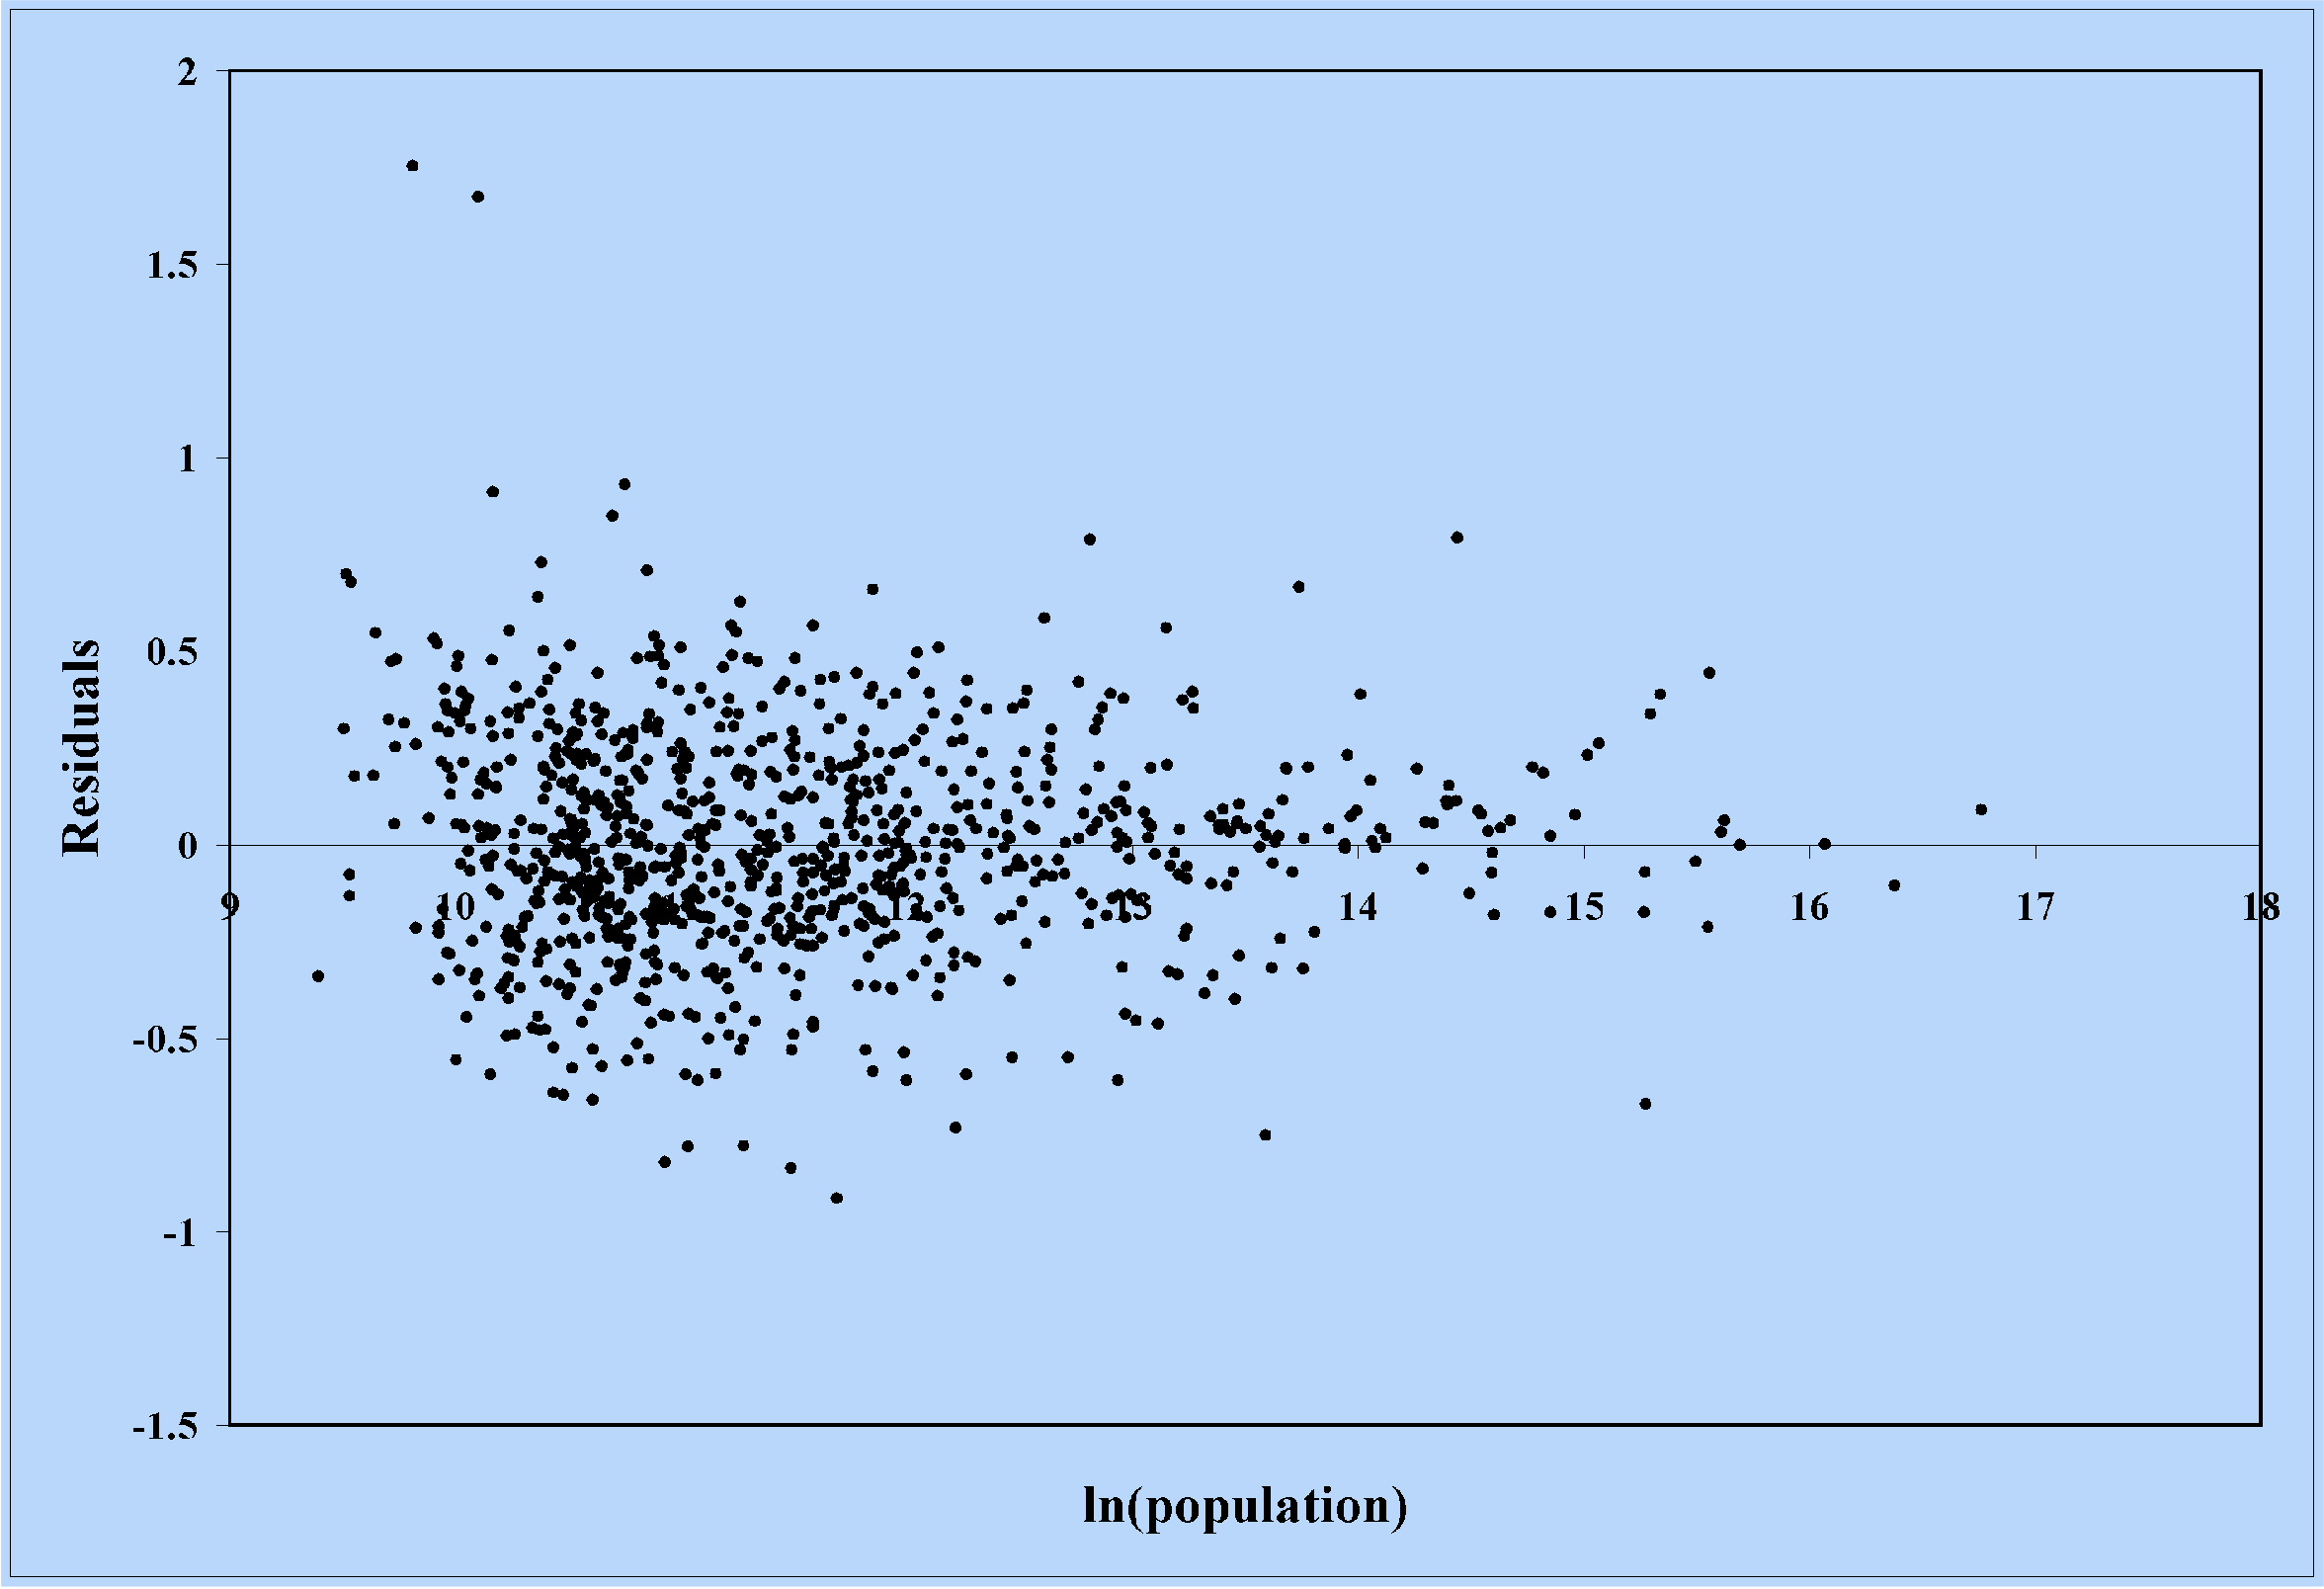
\includegraphics[scale=0.30]{fig/residuals-lobo.png}
\caption{Residuals from regressing ln(total wages) on ln(population) using data for all 943 urban areas of the United States showing larger unexplained components for smaller cities. \cite{loboUrbanScalingProduction2013}.}
\label{fig-residuals-lobo}
\end{figure}



\section{Conclusion}
 The dominant effect of financialization is to shift ownership of housing from occupiers to owners of financial capital. In this chapter, we have described a number of the most likely channels through which the effect of financialization on ownership  might be transmitted through the economic and social body of of the city to the Alonso-Jacobs cycle, where agglomeration effects generate wealth. The list is not complete but it provides a framework for testing the model's sensitivity to a range of policy interventions and lays the foundation for empirical work.  

The key result is that both our analysis and our simulations indicate that finacialization   can affect urban productivity. 

Financialization may also affect the industrial structure and the settlement pattern as well, but we defer extending the model to include these effects. Our focus in this chapter has been limited to examining possible channels through which the housing market financialization is likely to affect to affect the productivity of a city. We conclude, based on our analysis and simulations,  that the unrecognized impacts of financialization of the urban housing market may have extremely serious effects on the economy as a whole.

% We have modeled the relationship between ownership and the inputs to the aggregate production function described in Chapters~\ref{chapter-growth} and \ref{chapter-model}. 

% {\color{red}
% Essentially, the discussion in this chapter has guided and helps explain the policy experiments we have conducted. MAYBE ADD A FINAL SENTENCE PULLING IT ALL TOGETHER?}





